\chapter{Software defined radio}
In this chapter, we take a brief look at the general concepts of
software defined radio and how these concepts compare to a regular
radio implemented in hardware. As the name implies, some parts of a
radio are implemented in software which provides flexibility and
efficiency in a variety of different radio applications. The
flexibility relates to radios that allow the software to be redefined
and therefore can, at any time, be reprogrammed to perform a specific
task. Software-updates to accomodate operating needs and improve
security are easy and they make the \gls{SDR} a cost efficient
solution, not only for development but also in deployed systems.

Some of the signal processing concepts presented in the previous
chapter are concepts that define the functionality of a radio. Mixers,
filters, amplifiers and modulators/demodulators are some of the
components that enable these functionalities in a radio. For a
\gls{SDR}, these components can be defined in software to accomodate
certain needs in different environments.

\section{General architecture}
The general characteristics of \gls{SDR} imply that the hardware
components must be configurable in software and that these components
handle the analog signal generation and sampling.

\begin{figure}[H]
  \centering
  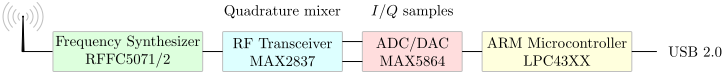
\includegraphics[width=.9\textwidth]{figures/sdr_hackrf_block_diagram}
  \caption{A roughly sketched example of HackRF One's architecture and
    its hardware components~\cite{hackrf_diagram}. A received signal
    is converted to a supported frequency range, separated into
    $I$/$Q$ signal components, then sampled and passed to a \gls{USB},
    interface at the microcontroller. The \gls{USB} interface allows the
    device to be configured and both receive and transmit data.}
  \label{fig:hackrf_block_diagram}
\end{figure}

\cref{fig:hackrf_block_diagram} roughly illustrates an example of how
a \gls{SDR} data pipeline could look, in this case the HackRF One. HackRF
One is an open source \gls{SDR} platform developed by the Great Scott
Gadgets team~\cite{gsg}.

The \gls{USB} standard provides a serial interface that is supported
by a wide range of machines and microcontrollers. With a
microcontroller, the configuration of hardware can be mapped by
low-level firmware and this leaves a simple protocol on the \gls{USB}
interface to communicate with the device. For signal generation and
sampling, parameters such as tuning frequency and signal gain may be
of interest to configure. These opportunities are what makes a
\gls{SDR} attractive and the device can be used for any application as
long as the hardware support the requirements e.g.\ frequency
spectrum, bandwidth and sufficient sampling rate.
